% to cite stuff use \cite{cite_key}

% Heirarchy:
%\part{part}	-1
%\chapter{chapter}	0
%\section{section}	1
%\subsection{subsection}	2
%\subsubsection{subsubsection}	3
%\paragraph{paragraph}	4
%\subparagraph{subparagraph}	5

\documentclass{article}
\usepackage{times}
\usepackage{cite}
\usepackage[autostyle]{csquotes}
\usepackage{marginnote}

%\textwidth = 490pt

\usepackage{graphicx}
\DeclareGraphicsExtensions{.pdf,.png,.jpg}
\graphicspath{ {./figures/} }

\begin{document}

\title{Bringing Knowledge Through AI and SMS}
\author{Sam Heather\\
  Department of Computer Science,\\
  The University of York,\\
  \texttt{sam@heather.sh}}
\date{\today}
\maketitle

\newpage

\begin{abstract}

\marginnote{It is early days so it is normal that many things are missing from the abstract. You should keep in mind that it should include later on few sentences on method/experiment, result and conclusion.}

In remote Africa, there are millions of disadvantaged and  uneducated individuals, who, in the vast-majority, do not have access to the internet and the access to knowledge that this brings.  Outside of their immediate friends and family, individuals can not get access to the information they need on anything from their own body to social problems.

In many parts of the world, the number of people without access to the internet, but access to a mobile phone, is significant.  This project aims to research and develop a system capable of bringing knowledge through a question and answer based interactive system, in the language natively spoken by the user, through the use of a simple Artificial Intelligence and an SMS interface.  The system will be expandable, such that it can be adjusted to handle questions on any knowledge area.

This project raises ethical issues relating to the responsibility of providing accurate information when in a position of trust, the ethics of machine translation and maintaining user privacy.
\end{abstract}

\newpage
\tableofcontents
\newpage
\listoffigures
\newpage
\listoftables
\newpage

\section{Useful thoughts from Lilian}
Take a quick look at list of other students previous projects to get an idea of how intro/lit review is structured etc.

Remember to take notes on when I come across problems, for my conclusion.

\section{Introduction}

\subsection{Background of this project}

The inspiration for this project originates from a project the author undertook in September 2014 whilst attending a week long 'hackathon' (Yacht Hack, http://toughhackers.com/yacht-hack-2014/), with Julie Markham and Nicholas Hopper, called Shy.  On this project, the author created a project to prototype a mobile application that would facilitate the immediate answering of questions that fall within certain categories.

A semi-functional prototype was completed for iOS (shown in Figure~\ref{fig:shy-ios-screenshots}, although question recommendations were evaluated without knowledge of previous material the user had viewed, and as such there was no knowledge of their interests to support explicitly targeted answers for a question they might search for.

Up until this point, the service was restricted to working on iOS smart devices only, with poor quality question/answer matching.

\begin{figure}[htb] 
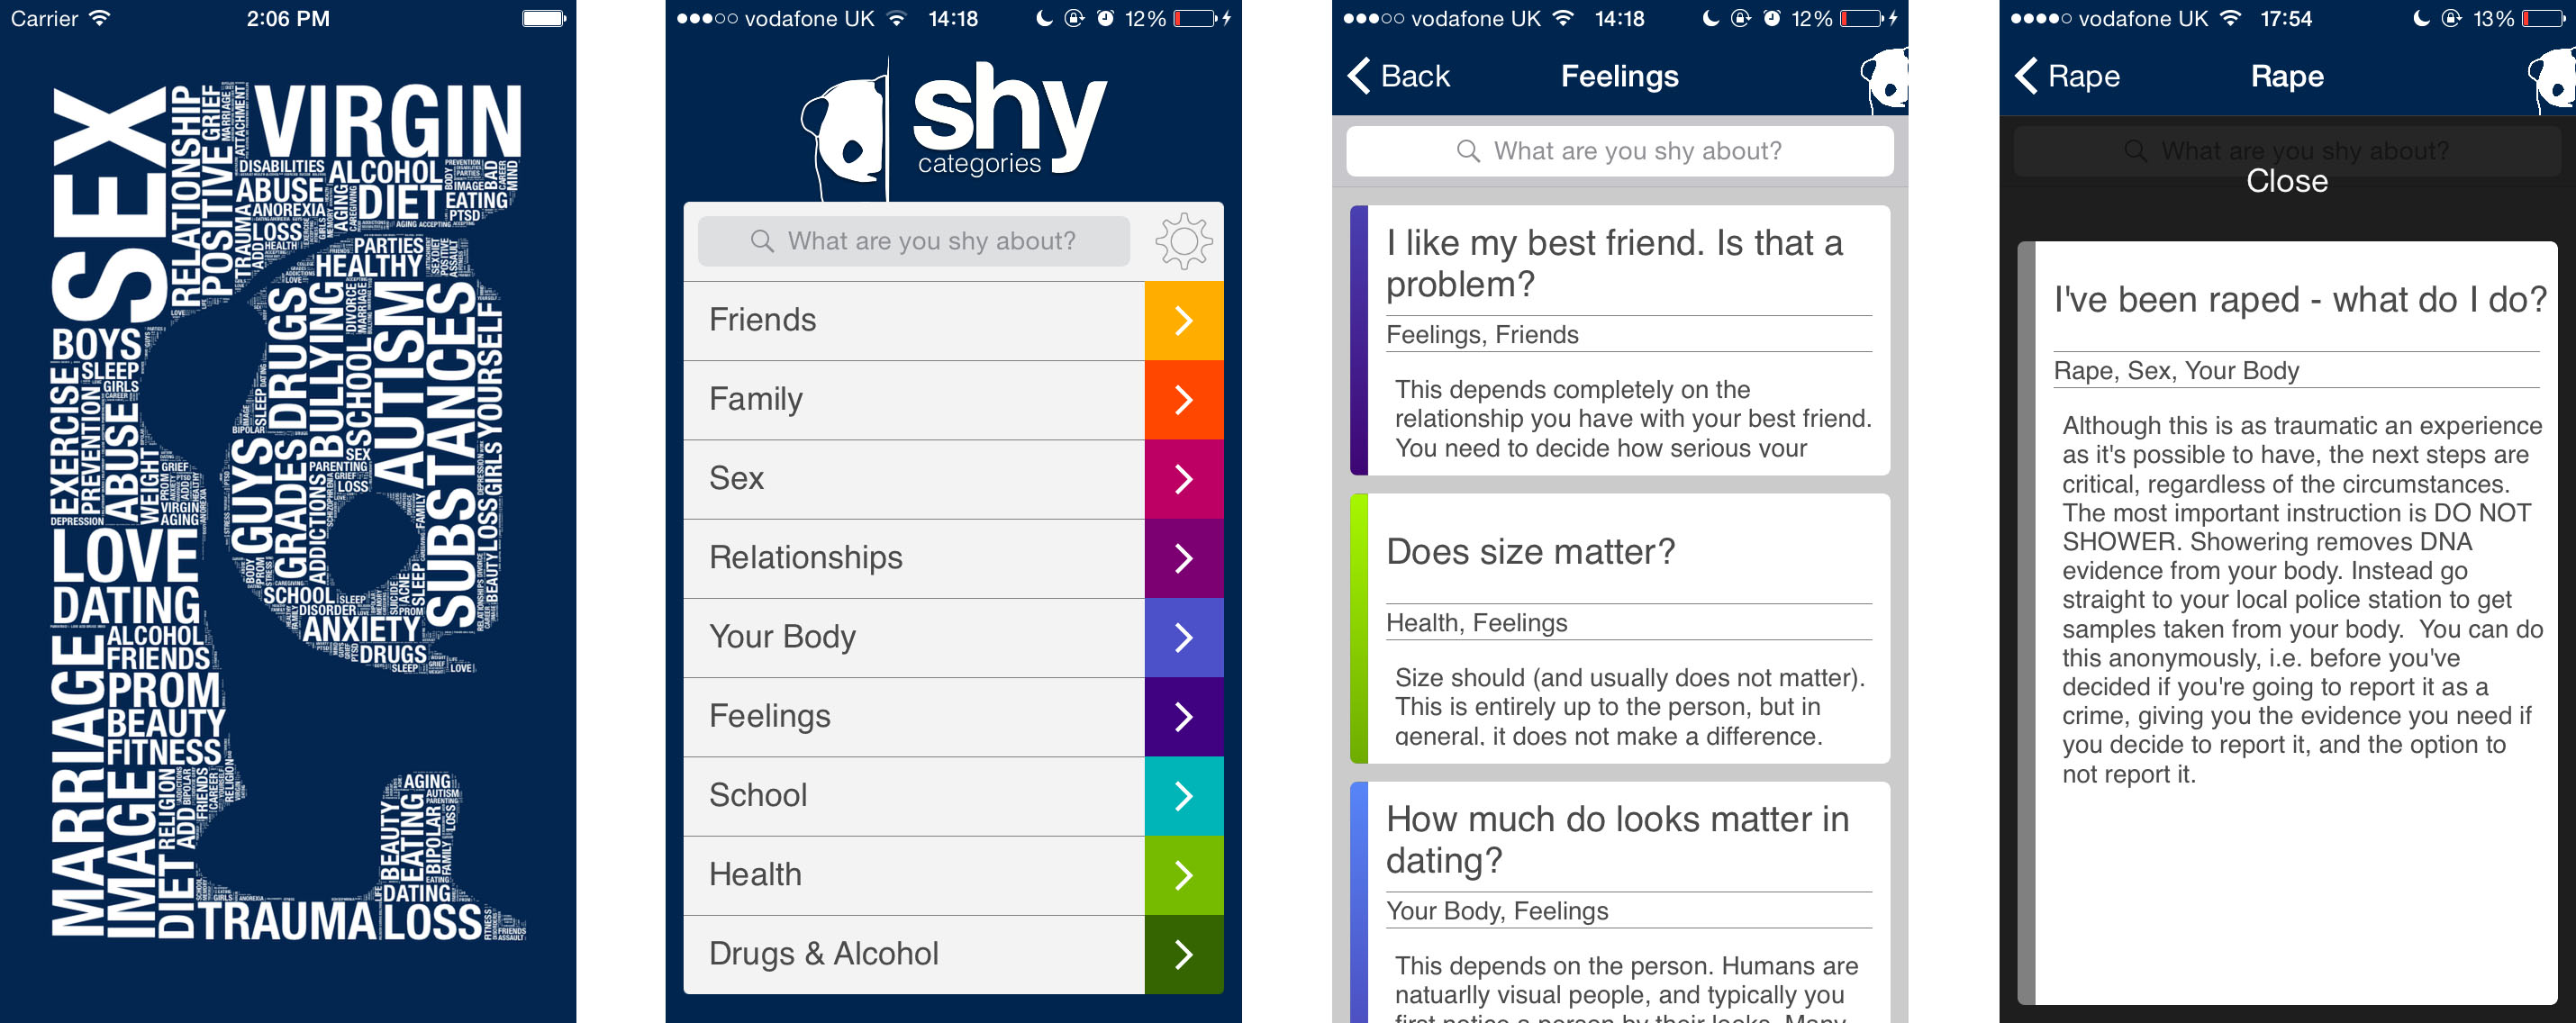
\includegraphics[width=\linewidth]{shy-screenshots}
\caption{Screenshots of Shy iOS App}
\label{fig:shy-ios-screenshots}
\end{figure}

\subsection{Motivation for this project}
Access to knowledge is, in the opinion of the author, a critical part of modern life.  It's also a Human Right, under the Article 27 of the Universal Declaration of Human Rights~\cite{community1948universal}.  Indeed, we use tools to access knowledge hundreds of times each day, often unaware that we are doing so.  Despite this, hundreds of millions of individuals live without this facility.  This project aims to investigate and create a technology to give more people access to knowledge, and thus their human rights.

The project also involves the use of a number of systems to work, including machine translation, an SMS input/output system and a custom system to build a profile on a user, to facilitate high-quality question-answer matching.  These, along with some complex ethics and privacy issues create an interesting project that draws together many technologies and discussions in a way that can be used as a basis for other projects in the future.

Computer software is an important tool for teaching as it encourages users to take a hands-on approach to learning, and provides some variation from traditional methods of teaching. JFLAP specifically was also found to increase the level of involvement for
Chapter 1. Introduction 3
students in a study by Rodger [2]. The University of York uses JFLAP in the teaching of a first-year Computer Science module on formal languages, and most students have found that the software has helped them to understand the processes behind the computational models involved (see Section 3.1.1.1). In addition, after having experienced the software as a user, there was a considerable incentive to extend the software to enhance the learning experience for users.

\subsection{Aims of this project}

The first goal of this project is to assess and address the ethical issues that arise from the software that this project aims to create.  These include the responsibility the software has, stemming from it's position of trust, to provide accurate information and protecting the privacy of users by using only necessary information, among others.  The author will do this by researching ethical issues relating to the technologies that the project will use, for example machine translation.  This will then be used to feed the design process of the software and to specify the expected use-case of it.  Finally, the resulting software will be evaluated through experimentation, with volunteers been asked to ask a set of questions within a topic area, in a non-English language, and evaluate the relevance of answers returned.

\subsection{Structure of this report}
This report starts with a review of pre-existing literature on this topic, in chapter~\ref{sec:literatureReview}, where the author looks at existing software, tools and services of a similar type to those that will be either used in this project or that which this project hopes to create to research the problems that they stumbled across.  Comparisons between different software development life-cycles are also discussed.

Chapter~\ref{sec:method} describes the method that will be taken to develop the software and service.  This covers the software development life-cycle that will be followed, and sets out a plan for when development will take place.  Requirements will also be identified, described and categorised  as either functional or non-functional.  A method of evaluating the success of the software will also be discussed and choosen.

The design of the software, driven from information collected from the requirements, will be set out in Chapter~\ref{sec:design}.  The individual components that make up the technology will be described and discussed\marginnote{described and discussed, or just described?}, followed by a description of how these modules will interface with each other to build a complete system.  

Chapter~\ref{sec:implementation} contains details about the implementation of the software.  This includes information on the tools that were used to create components such as the SMS interface and question/answer matching system.

Results from the evaluation of the system will be presented in Chapter~\ref{sec:results}.  A discussion of these results and their implication on this project is presented to the reader in Chapter~\ref{sec:discussion}.

Finally, a conclusion is made in Chapter~\ref{sec:conclusion}.....
\marginnote{ Lilian: How should my conclusion/evaluation be presented?  I thought it should be an evaluation section, with a conclusion of the evaluation as a subsection, but this doesn't follow the structure we briefly discussed in our last meeting?}

% Lilian: This section should be expended, especially mentioning the consequences of such assumptions. Why do you make those assumption (e.g. time constraint, little or no consequences, ...). What limitation this may cause to your findings.  Shows a mastery of the field.
\subsection{Assumptions Within This Project}
This project will make the assumption that users of this service have basic literacy skills in a language supported by the project.  Although this is not true for the whole of Africa, expanding the remit of this project to include a 'graphical' user interface that works over SMS is a challenge larger than would fit in an undergraduate dissertation.

\newpage

\section{Literature Review}
\label{sec:literatureReview}

{\bf The point of this is to show that I 'own' the material and subject (competence).  Show different points of view, choose a side, express a view on which I prefer and if I agree, critique.  Have objective goals.}

% expand introduction to explain why sms, then look at related work in next section.  compare to smart phones loosely.
A significant amount of work has previously been undertaken in the area of making knowledge quickly accessible to us in the form of questions and answers.  To take one example, consider the situation of suspecting that a relative was suffering from a disease, for example, Cholera.  The initial step would be to search for information before seeking medical assistance.  In the connected world, this is easy - a simple Google search returns the answers, as shown in Figure\ref{fig:cholera}.

\begin{figure}[htb] 
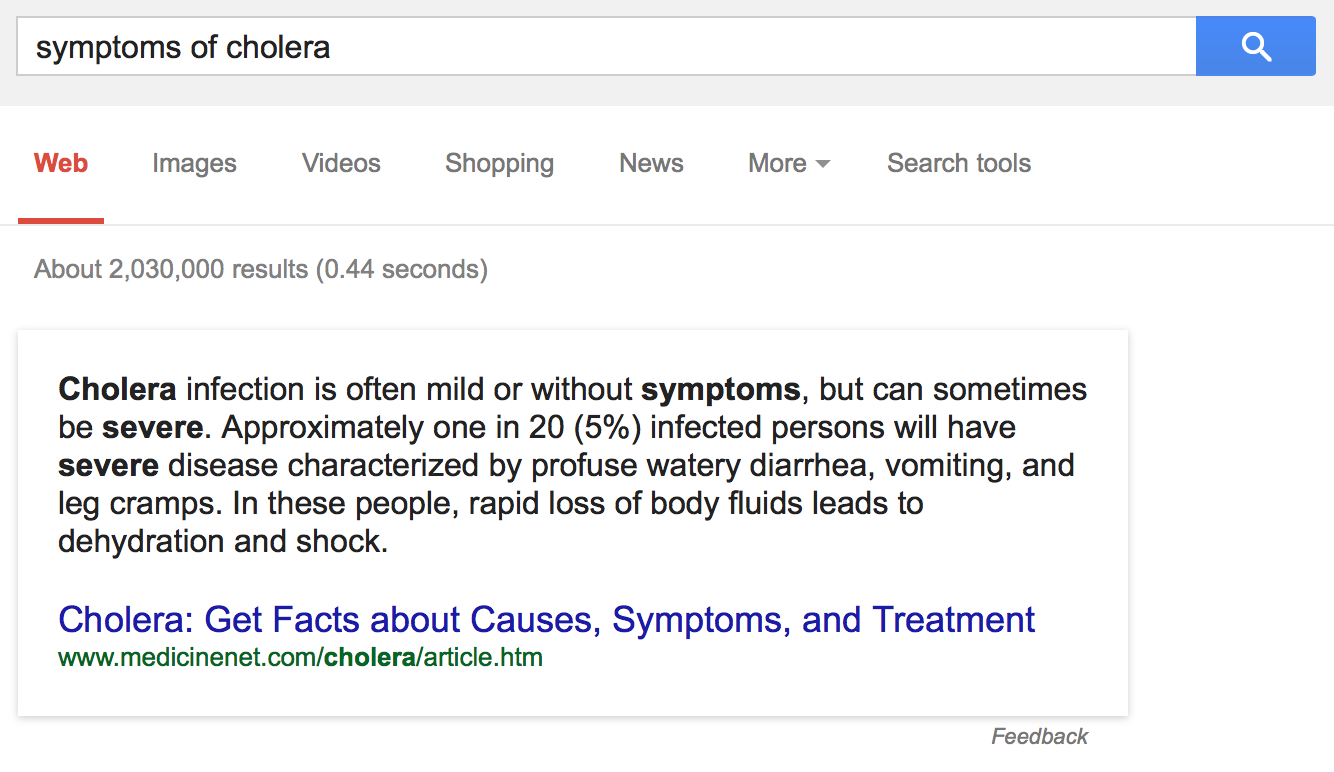
\includegraphics[width=\linewidth]{googleCholera}
\caption{Google Now information box}
\label{fig:cholera}
\end{figure}

% Lilian: You should give a caption to all figures and tables. use \label{fig:WebQuery} after \caption{Web query result for "Symptoms...}  for example. In this instance you should mentioned the date you made the query and which search engine you have used.

This is easy to do in the developed world, where up to 75\% of the population are connected to the internet~\cite{ITU_Cell_Usage_2013} (with the population of elderly people been largely responsible for the remaining 25\%~\cite{Gov_Internet_Usage_UK_2014}).  This contrasts strongly with the situation in the African continent, where, in 2013, internet usage had only reached 16\%~\cite{ITU_Cell_Usage_2013}, a figure largely inflated by South Africa, where 5\% of the African population generate 2/3 of internet traffic from the African Continent~\cite{ITU_Cell_Usage_2013}.

% But there are other communication methods which are proven to work
\subsection{Previous work using SMS}
Although the above suggests that the African continent is majoritively disconnected, this is not the case.  Because of restrictions in the electricity available, the ways in which a mobile phone can be used in Africa have far surpassed those in the developed world ~\cite{Fox:2011:Online}.  Interesting such examples include automated services which SMS HIV/AIDS sufferers, reminding them of medication to take, and providing access to current market information for agriculture and farming, saving farmers from making daily trips (often many kilometres) or relying on out-of-date information from a weekly radio broadcast ~\cite{Aker_Mobile_Phones_2010}.

Interactive systems have also been developed to operate over SMS.  One successful example includes mobile money platforms.  These allow for users, from any background, to pay and be paid for goods, and to transfer money across long distances, at negligible cost ~\cite{Aker_Mobile_Phones_2010}.  One of the most highly adopted services is M-Pesa - which, in Kenya alone, was responsible for £5.7 Billion in transfers in 2012 \footnote{Data from Safaricom, M-Pesa operator in Kenya - actual value 817,085,000,000 Kenyan Shillings, converted to GBP on 1st November 2014 at rate of approximately 0.007.}.  M-Pesa gives users a balance linked to a national ID number, from which they can pay for goods by sending an SMS with a cashier (recipient) number or pay outstanding bills in a similar way.  Non-subscribers can also use the system, by depositing money with a M-Pesa cashier in exchange for an access code, which can be sent via SMS to a contact, who can subsequently redeem it with their local cashier~\cite{Aker_Mobile_Phones_2010}.

This difference in standard use of cell phones is demonstrated in the International Telecommunications Unions's 2013 report, which shows that in Europe, for 790 million mobile subscriptions, 53\% of subscribers have mobile internet access (422 million), compared to 17\% in Africa (93 million have mobile broadband, out of 545 mobile subscribers).  This is due to the prohibitively high cost of accessing data services, regardless of the hardware that the user has.  \footnote{In 2012 in Europe, 500 MB of data per month for 12 months cost 1.2\% of the average Gross National Income Per Capita (GNI pc).  In Africa, the average price was 30x this, at 36.2\% of an individuals GNI pc.  ~\cite{ITU_Information_Society_2013}}

% No research has been undertaken investigating whether bringing knowledge through this method is viable option.

\subsection{Ethical Issues}
This project raises a swathe of ethical issues related to translation accuracy, providing information to people in an ethical way and maintaining user privacy.

\subsubsection{Ethics of Providing Information}
One significant issue for this project stems from providing information that may affect an individual or lead them to take a harmful action.  In a similar way to that which a teacher has a responsibility to teach accurate information to a pupil, due to their position of trust, any service relied upon by a user must equally provide accurate information.  The result of not doing this could be providing inaccurate information that leads to a user carrying out an action that causes harm.

% Lilian: You may want to look toward news paper (online/printed) to look at current/past issues that led to a law suit/inquiry and subsequent verdict/laws that may have been changed.

% Lilian: You should provide both point of view so do use this material, then you will have to critic both point of views. 
{\bf this needs to be waaaayyyyy expanded, but I struggled to find information that was useful.  There's lots on remote education, and on basic ethics of teaching, but I struggled to find anything specifically relating to ethics of ensuring information you provide is correct (actually I found some material that pointed the other way)}.

\subsubsection{Ethics of Translation}
A significant part of this project is represented by the support of multiple languages.  It is clear that translation on demand, at scale, needs to be automated by some kind of machine or algorithmic translation.

This project involves two blocks of translation.  These are:
\begin{itemize}
  \item The translation of the user's input into the language of the system (English)
  \item The translation of the answer to a users question from the system language to their local language.\ldots
\end{itemize}
The second of these raises some issues.  To understand these, it is necessary to first understand the two categories of machine translation.

Rule-based machine translation effectively treats human language in a similar style to programming languages.  Formal grammars and lexicons are used to represent words that exist in either the source or target language, structures representing the translation of individual words or groups of words.  Map structures map individual or groups of words to their translated counterparts, sometimes with multiple results (a 1-many map), from which rules decide which is selected.  Maps and rule sets are created by trained computational linguists~\cite{kenny2011ethics}.

More commonly, Statistical Machine Translation (SMT) is used (for example, this is used by Google and Microsoft Bing Translate)~\cite{kenny2011ethics, Google_Translate_Research}.  Statistical machine translation learns maps between strings of words of potentially non-equal lengths from pre-existing original texts and their trusted human translations.  The accuracy and breadth of language support for translation increases as more source material is analysed by the system, as potentially erroneous or low quality translations can be identified and marked.  SMT is also dependent on the quality of the human translation on the input material ~\cite{kenny2011ethics}.

The aforementioned issue that is present in statistical machine learning systems comes from the knowledge we assume an individual has and derives from a word.  In human translation, this is solved by the translators knowledge of the difference in material culture, allowing them to append necessary information to the resulting translation that the recipient might find useful.  In statistical machine learning, cultural awareness of material knowledge is a separate problem on it's own, on this scale.  {\bf formal reference to this, probably again from Kenny, but should be able to find better}.  To take one example, from Melby (2006),

\blockquote{"when translating a French menu, a human translator might stop to think that an English speaker in France would appreciate being told that a steak tartare is served entirely raw, even if this information is not contained in the original text (because French people might be assumed to know this already). Such a translator would be aware of differences in material culture, and would be able to empathise with the English speaker who might choose to avoid the dish, given more information"~\cite{melby2006can, kenny2011ethics}}
\marginnote{Lilian: quote taken from ~\cite{kenny2011ethics}, but quote is interpreted from ~\cite{melby2006can} - so I think referencing both is correct, but for this reason rather than last reason we discussed?}

This issue is a result of the translation engine not been capable of taking as input, and using, a complete representation of the expected cultural differences between those who speak the input language and those who speak the output language~\cite{melby2006can}.

{\bf below should really be expanded and be in the discussion.  Explain the decision to keep translated answers in the database, which are pre-approved, to ensure no cultural misunderstandings.}

Because the potential use of this system, regardless of whether this is within this project or by a third-party using the results of this project upon completion, could include distributing information that may be used by an individual making an important decision, cultural confusion such as this could have potentially catastrophic effects.

\subsubsection{User Privacy and Data Protection}
Privacy is a significant part of this project, since the

\subsection{Software Design Life-cycles}

\newpage
\section{Method and Requirements}
\label{sec:method}

\newpage
\section{Design}
\label{sec:design}

\newpage
\section{Implementation}
\label{sec:implementation}

\newpage
\section{Results}
\label{sec:results}

\newpage
\section{Discussion}
\label{sec:discussion}
This section's content...

\subsection{Protecting the Identity of Users}
This subsection's content...

\subsubsection{The Purpose of a Non-reversible Hash}
This subsubsection's content...

\newpage

\section{Conclusion}
\label{sec:conclusion}

\newpage

\section{Extending this project}
If the author was able to expand this project, areas for expansion include:
\begin{itemize}
  \item Addressing the issue of literacy
  \item Automating the expansion of the database \ldots
\end{itemize}

\newpage

\bibliography{mybib}{}
\bibliographystyle{plain}

\section{Appendix 1 - Data usage}

\end{document}  %End of document.